\section{How does git work internally?}

To understand how git works we need to know some basic commands.

\subsection {Basic local commands}

As any other VCS git stores its data in the repository directory.
There are two major ways to get a repository.
One would be by simply creating a new empty git repository in your directory of choice:
\begin{lstlisting}
$ git init
\end{lstlisting}
This command creates a new subdirectory .git/ where all your version control
data is stored. \cite{gitinternals2008} p 55 \\
The second is to clone an existing repository over an URL. Possible protocols
are FILE SSH HTTPS HTTP or GIT. Of course on the target location must host a
git repository:
\begin{lstlisting}
$ git clone 
    git://github.com/rails/rails.git
\end{lstlisting}
Git will clone the whole ruby on rails project from github and we're
ready to get to work. \cite{gitinternals2008} p 56 \\

After we have a new repository we can add some content:
\begin{lstlisting}
$ touch README
$ git status
$ git add README
$ git commit -m "Added README file"
\end{lstlisting}

This code produces an empty README file. The status command displays any change
of the repository. There we can see that the README file has been added and we
track this file simply by telling git to add the file to the index. Additionally
git now stages the file, but we are going to cover the staging feature later in the next
section. Then we commit the changes with a short and descriptive message. After
this git stores the changes into the repository and points the default master
branch to the new commit. \cite{gitinternals2008} p 55 \\

\subsection{Git over network}

After there has been committed a huge amount of work in the local ruby on rails
repository we can share the work telling git:

\begin{lstlisting}
$ git push origin master 
\end{lstlisting}

This command will only succeed if you have the appropriate access rights to the
project. But if we had them, the master parameter tells git to take the default
branch and transmit the changes to the host. We could also specify any other
branch and transmit it to the destination host. \\ 

Also one should know that the origin parameter is our destination. You can
simply add many different socalled remotes:

\begin{lstlisting}
$ git remote add [name] [url]
\end{lstlisting}

This command links a short name to any url and you can share your
work over any network git is designed for. \cite{gitpro2009} chapter 2.9 \\

The last very important command is:
\begin{lstlisting}
$ git fetch origin
\end{lstlisting}

The fetch command is used to get work from other people of your project since
the last time you fetched. Very important is that this command does not
automatically merge the new updates into your local master branch. It just
downloads the updates and creates a new brach FETCH\_HEAD. Then you have to
manually merge the branch FETCH\_HEAD to the desired branch. 
If you dont need this very powerful feature you can simply execute:
\begin{lstlisting}
$ git pull origin
\end{lstlisting}
Git will automatically merge the changes into your master branch.
\cite{gitpro2009} chapter 2.9 \\

\subsection {Staging}

Now that we convered the fundamental basics of git. We can take a deeper look at
some parts of the logic used by git. One high level feature of git is the
\emph{interactive adding}. We create a new repository and add a file and commit
it. If we modify the same file again and try to commit with the command above,
git will not apply the modified file to the repository. This is because this file is
not explicitly added to the socalled staging mode. You have to explicitly add
the modified file to the staging mode and commit. This feature gives you much
more control over what goes into your repository or not. This feature is often
ignored and you can simply commit a unstaged file with this command:

\begin{lstlisting}
$ git commit -a -m "message"
\end{lstlisting}

The parameter \emph{-a} automatically adds the file to the staging mode and
commits it. \cite{gitpro2009} chapter 2.2

The picture taken out of the git pro book illustrates how files change their
lifecycle modes:

\begin{figure}[h]
  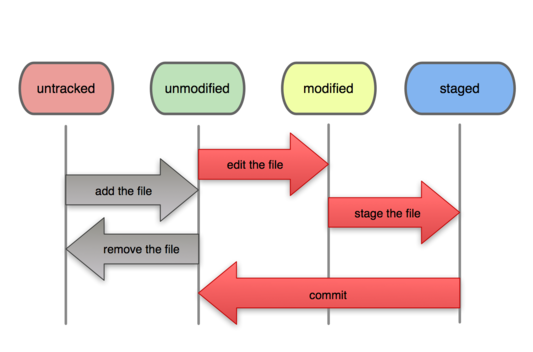
\includegraphics{img/file_status_lifecycle}
  \caption{File status lifecycle}
  \label{fig:File status lifecycle}
  \cite{piclifecycle}
\end{figure}

As we can see there are four modes a file can have. First we have to track them
once to get them into the lifecycle. If we modify we can use \emph{-a} on the
commit command to automatically stage and commit them, or we can take alot more
of control of our repository and stage them manually and avoid mistakes and
redundant changes that do not belong to a certain commit.
We can simply get information about the mode using the git command
\emph{status}. \cite{gitpro2009} chapter 2.2

\subsection {What makes git to a DVCS?}

Linus Torvalds did a quite good job to summarize what distributed means:

\zitat{Being distributed very much means that you do not have one
central location that keeps track of your data, no single place more important
than any other place \ldots } \cite{linustorvaldsgoogletalk2007}

Nearly all commands that git offer you are local operations. There is no need to
have any network connection at all to work on your project and track changes
afterwards. Moreover the whole history of your project is contained in your
local repository. Also all contributors of one project have that history if
they pull from you. Hence no repository has more information about the project
than the other.
